\section{Jouabilité \& Visuels}
\subsection{Sauvegarde}
\begin{frame}{Jouabilité}
\frametitle{Avancée du joueur}
\setlength{\parindent}{5ex}
Script principal
\begin{center}
\begin{tabular}{|c||c|}
\hline
    \textbf{Variables} & \textbf{Type} \\
\hline
    Point de sauvegarde actuel & Vector3 \\
\hline
    Objets & List<Objet> \\
\hline
    Statut de l'environnement & List<Environnement> \\
\hline
\end{tabular}
\end{center}
\end{frame}

\begin{frame}{Gameplay}
\frametitle{Avancée du joueur}
\setlength{\parindent}{5ex}
Base de données
\begin{center}
\begin{tabular}{|c||c|}
\hline
    \textbf{Variables} & \textbf{Type} \\
\hline
    Coordonnées & Dictionary<string, Vector3> \\
\hline
    Noms objets & Dictionary<string, int> \\
\hline
    Noms environnement & Dictionary<string, int> \\
\hline
\end{tabular}
\end{center}
\par Les classes Objet et Environnement héritent toute les deux de la classe Identifiant
\end{frame}


\begin{frame}{Gameplay}
\frametitle{Avancée du joueur}
\begin{figure}[H]
\centering
\begin{minipage}{.5\textwidth}
  \centering
  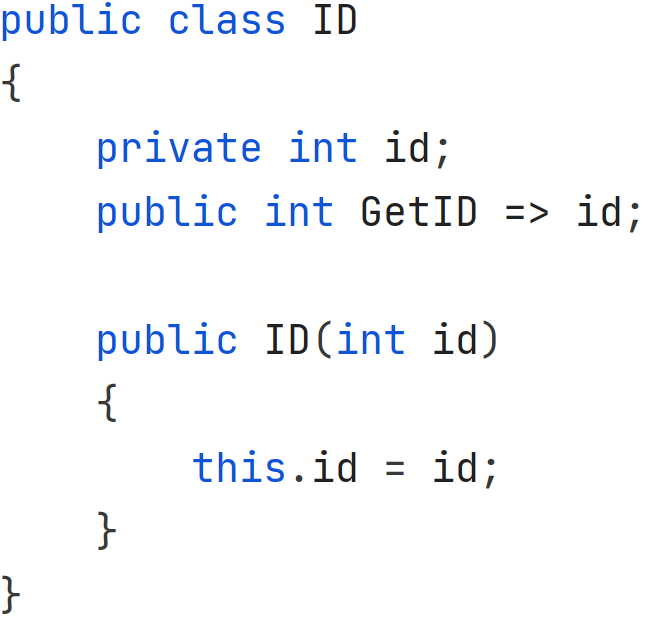
\includegraphics[width=.7\linewidth]{img/gameplay/IDclass.PNG}
  
  \caption{Classe Identifiant}
  \label{fig:ID}
\end{minipage}%
\begin{minipage}{.5\textwidth}
  \centering
  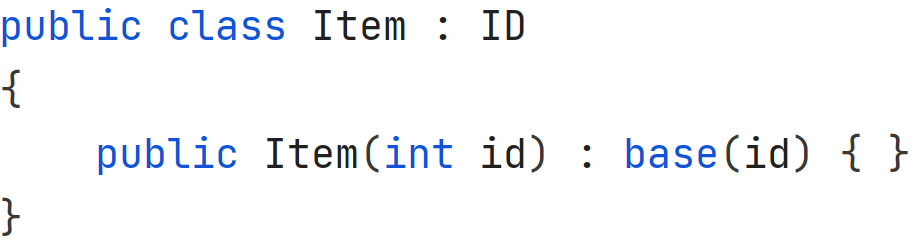
\includegraphics[width=.9\linewidth]{img/gameplay/ITEMclass.PNG}
  \caption{Classe Objet}
  \label{fig:Item}
\end{minipage}
\end{figure}
\end{frame}


\begin{frame}{Gameplay}
\frametitle{Sauvegarde des données}
\begin{description}
  \item[$\bullet$] Utilisation du format JSON\footnote[1]{ JavaScript Object Notation}
  \item[$\bullet$] Utilisation du chiffrement XOR\footnote[2]{ Signifiant exclusive OR / OU exclusif en français}
\end{description}
\end{frame}



\begin{frame}{Gameplay}
\frametitle{JSON}
\setlength{\parindent}{5ex}
Exemple de fichier JSON :
\newline
\newline
{"currentSave":{"x":50.0,"y":0.0,"z":100.0},"item":[{"id":101},{"id":102}],"env":[{"id":201}]}
\end{frame}

\begin{frame}{Chiffrement XOR}
\frametitle{Sauvegarde des données}
\begin{minipage}{.3\textwidth}
  \centering
  Table de vérité OU exclusif:
  \newline
  \newline
    \begin{tabular}{|c||c||c|}
        \hline
        \textbf{A} & \textbf{B} & \textbf{A XOR B}\\
        \hline
             0 & 0 & 0 \\
        \hline
            0 & 1 & 1 \\
        \hline
            1 & 0 & 1 \\
        \hline
            1 & 1 & 0 \\
        \hline
    \end{tabular}
\end{minipage}%
\begin{minipage}{.7\textwidth}
  \centering
  Exemple de chiffrement XOR:
  \newline
  \newline
    \begin{tabular}{|c||c||c||c||c||c||c||c|}
        \hline
            \textbf{Message} & M & E & S & S & A & G & E\\
        \hline
            \textbf{Clé} & C & L & E & C & L & E & C \\
        \hline
           \textbf{Message chiffré} & SO & HT & SYN & DLE & CR & STX & ACK\\
        \hline
    \end{tabular}
  \label{fig:xor}
\end{minipage}

\end{frame}

\subsection{Interaction}
\begin{frame}{Gameplay}
\frametitle{Action ''utiliser''}
\begin{description}
  \item[$\bullet$] Permet d'interagir avec l'environnement
  \item[$\bullet$] Assigné à la touche ''E''
  \item[$\bullet$] Divisé en deux scripts:
  \begin{itemize}
      \item [] Interacteur : Lié au joueur
      \item [] Interactif : Lié aux objet dit ''interactifs''
  \end{itemize}
\end{description}
\end{frame}


\begin{frame}{Gameplay}
\setlength{\parindent}{5ex}
Interacteur (dans l'ordre)
\frametitle{Action ''utiliser''}
\begin{description}
  \item[1.] Utilisation du Raycast\footnote[1]{ peut être traduit par ''lancé de rayons''}
  \item[2.] Aucun objet ne bloquant l'action
  \item[3.] Vérification de l'appui de la touche assignée\footnote[2]{ Rappel : touche ''E''}
\end{description}
\frametitle{Action ''utiliser''}
\par Interactif
\begin{description}
  \item[$\bullet$] Contient un évènement Unity
\end{description}
\end{frame}

\subsection{Chapitres 1 et 2 - Forêt}
\begin{frame}{Chapitres 1 et 2 - Forêt}

\begin{figure}[H]
\centering
\begin{minipage}{.5\textwidth}
  \centering
  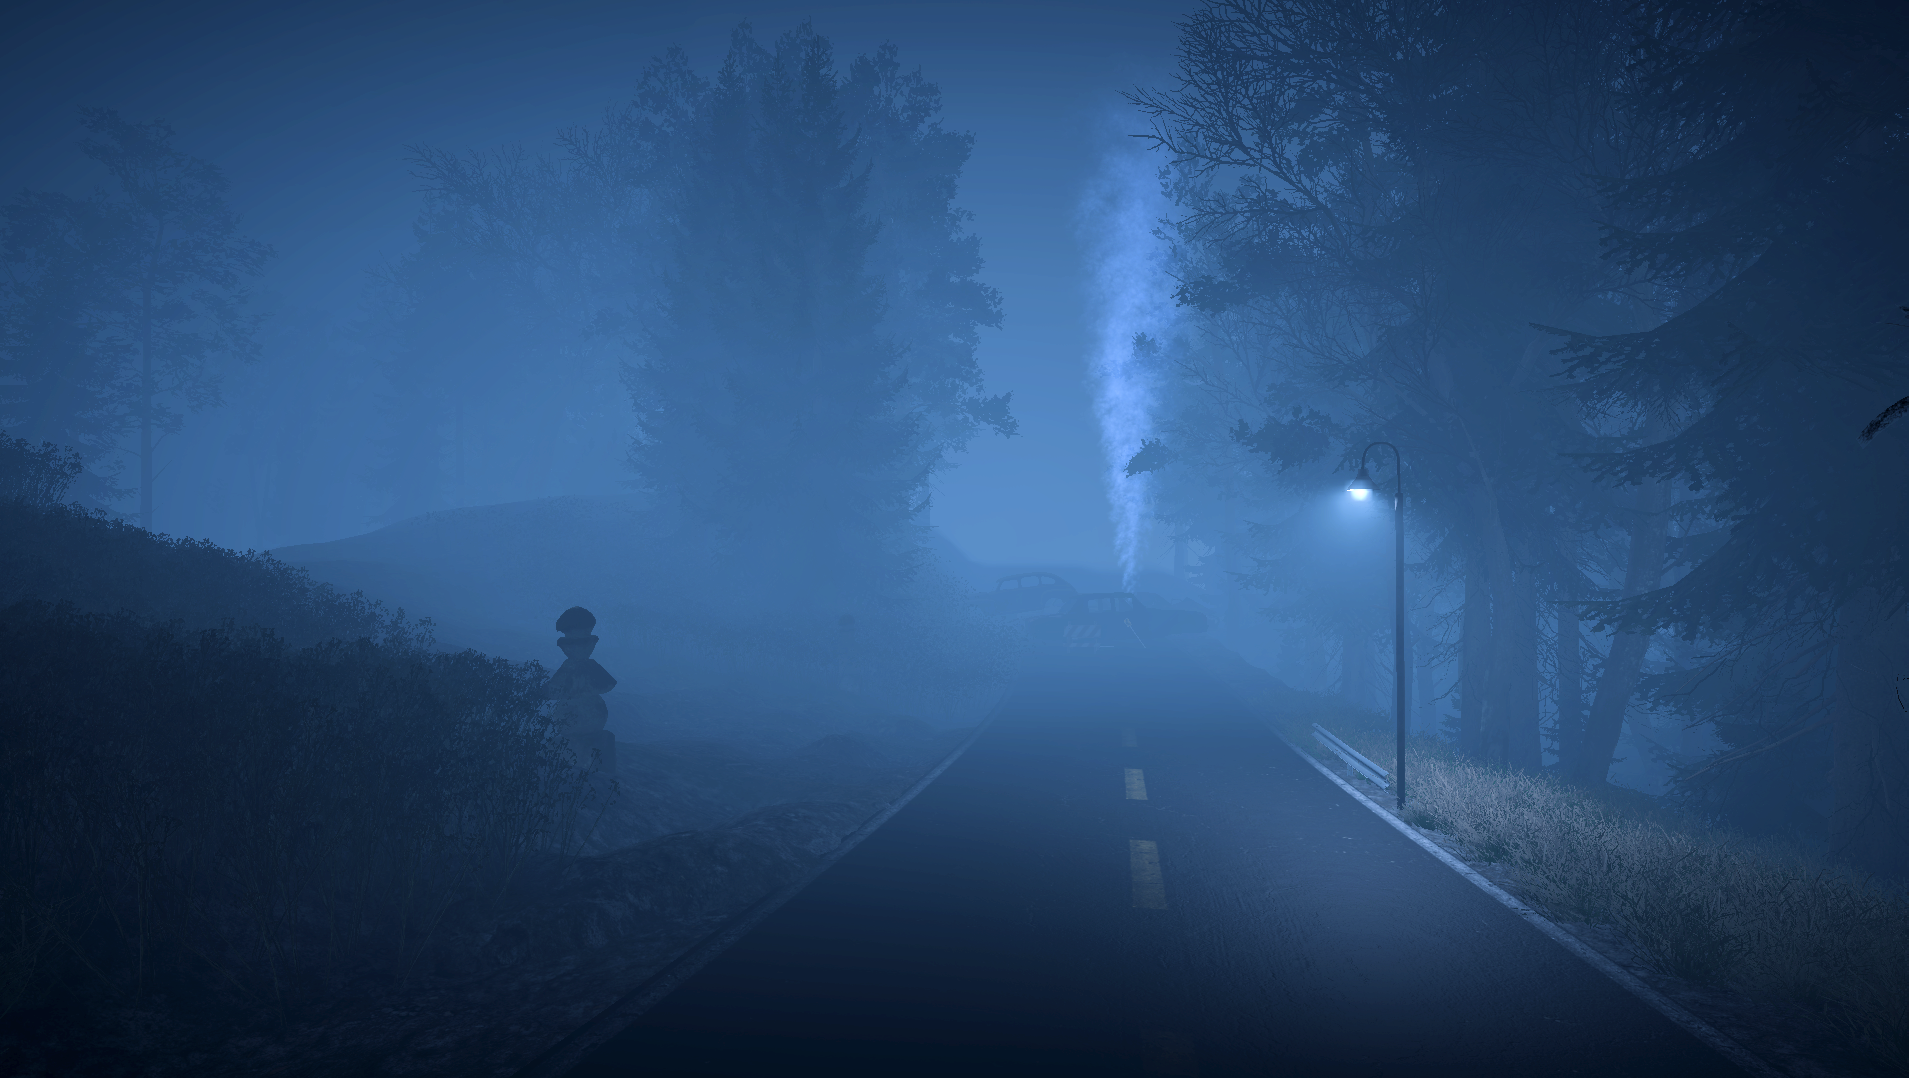
\includegraphics[width=.9\linewidth]{img/gameplay/hallo/spawn.png}
  \caption{Lieu d'apparition du/des joueurs}
  \label{fig:spawn}
\end{minipage}%
\begin{minipage}{.5\textwidth}
  \centering
  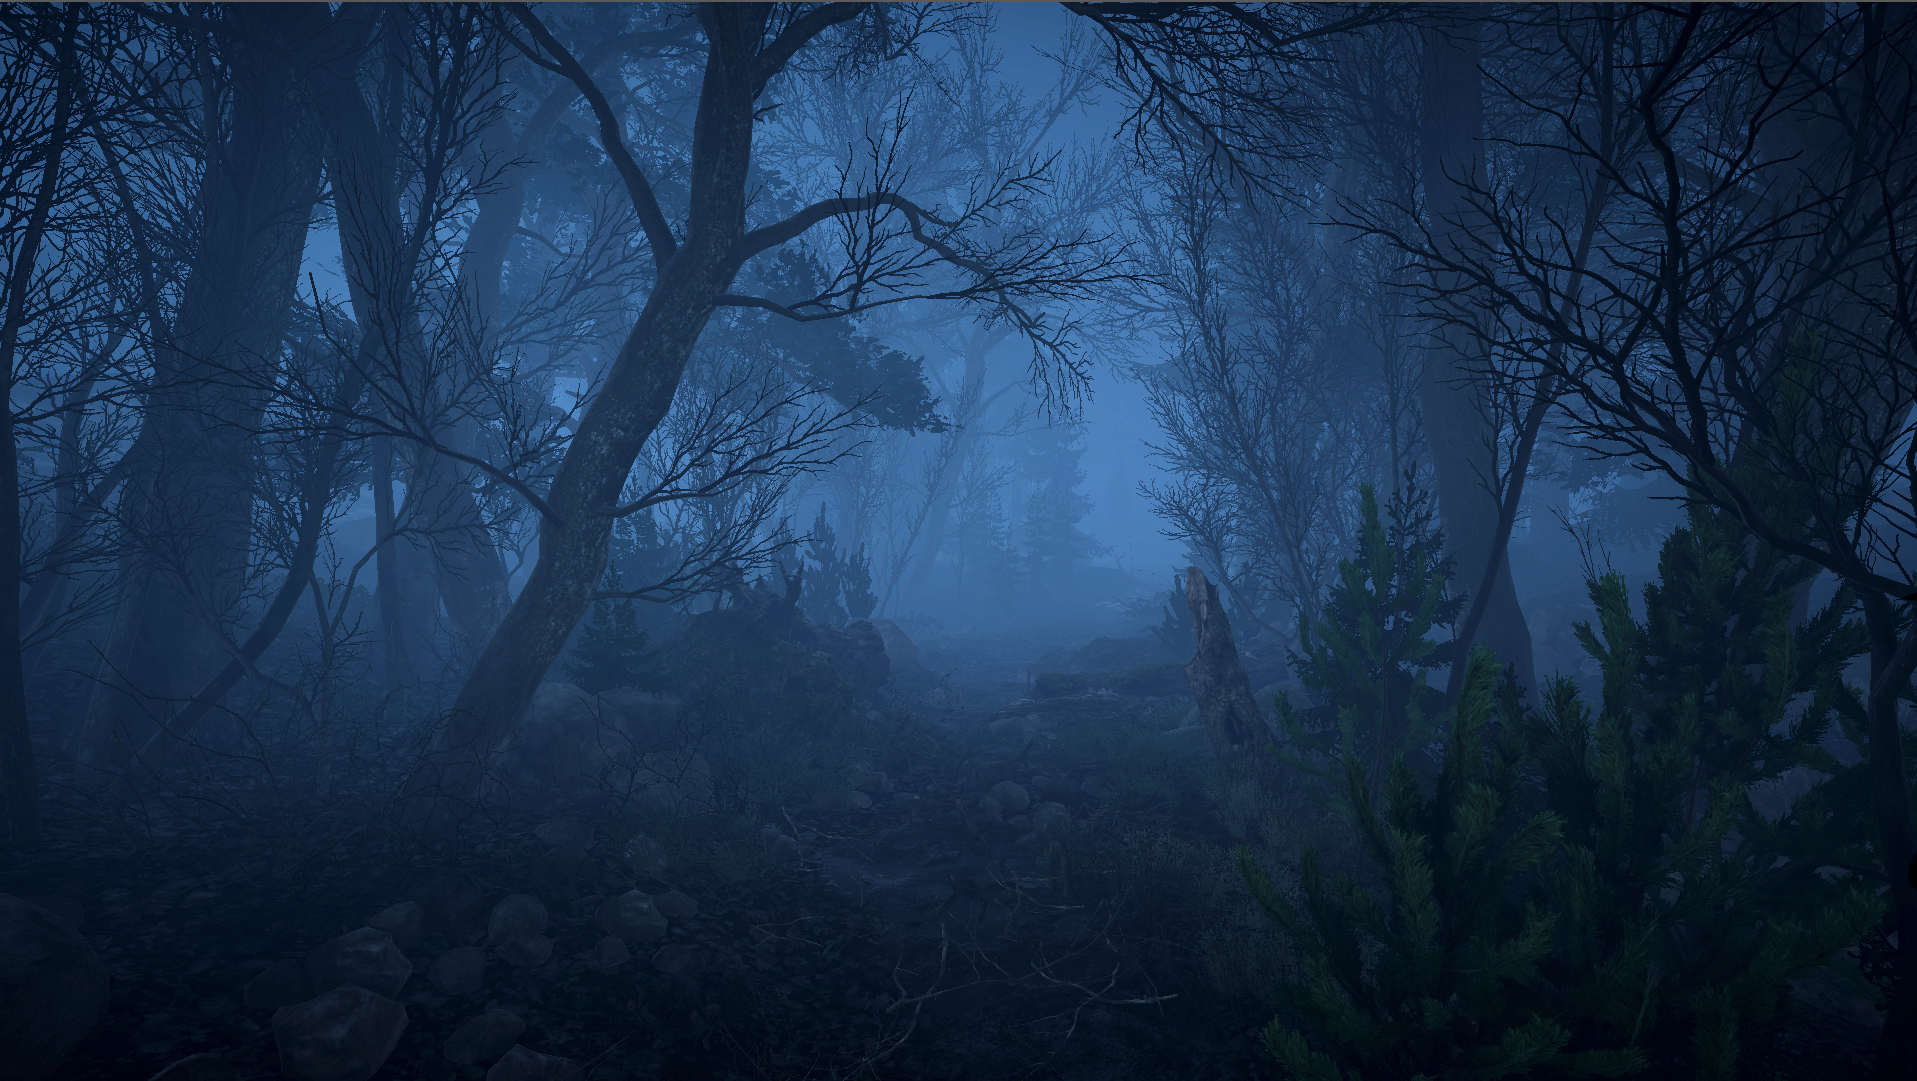
\includegraphics[width=.9\linewidth]{img/gameplay/hallo/forest.png}
  \caption{Forêt}
  \label{fig:forest}
\end{minipage}
\end{figure}
\end{frame}

\begin{frame}{Chapitres 1 et 2 - Forêt - Suite}
\begin{figure}[H]
\centering
\begin{minipage}{.5\textwidth}
  \centering
  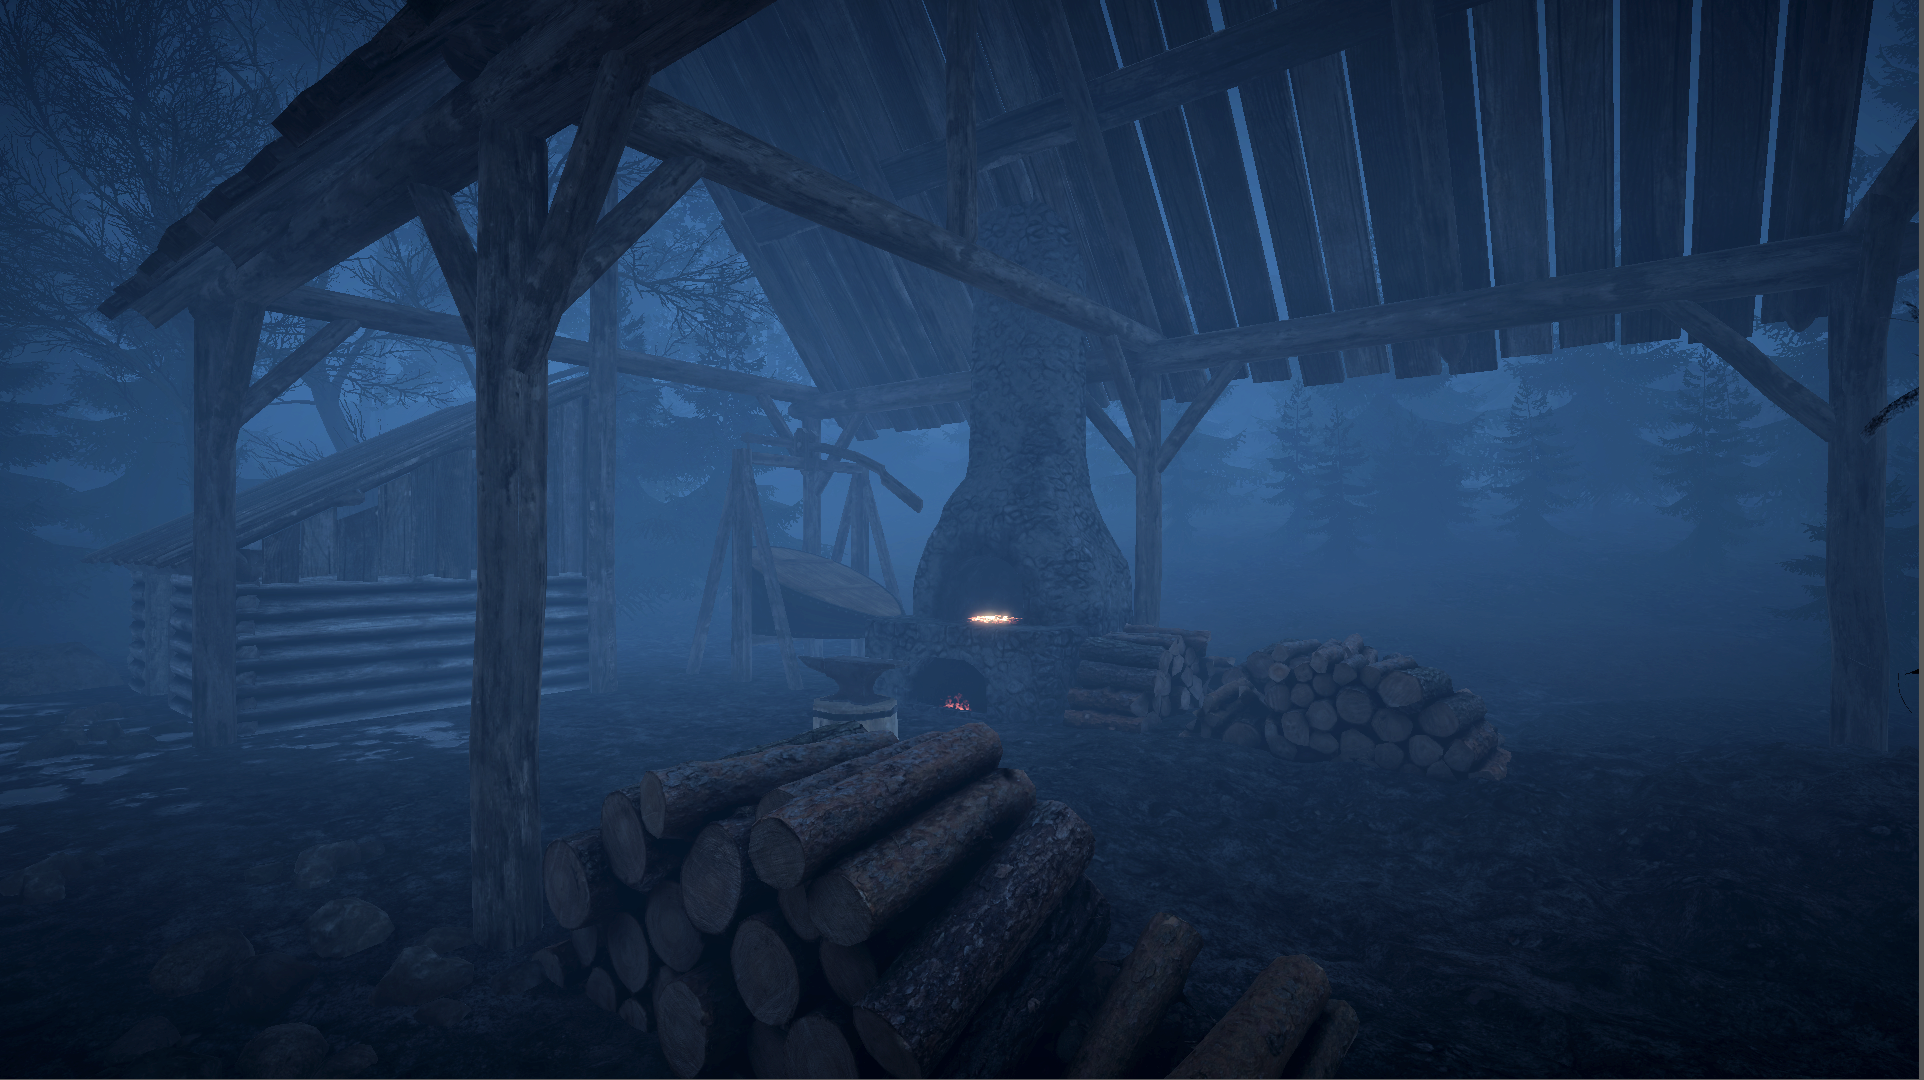
\includegraphics[width=.9\linewidth]{img/gameplay/hallo/house.png}
  \caption{Maisons}
  \label{fig:houses}
\end{minipage}%
\begin{minipage}{.5\textwidth}
  \centering
  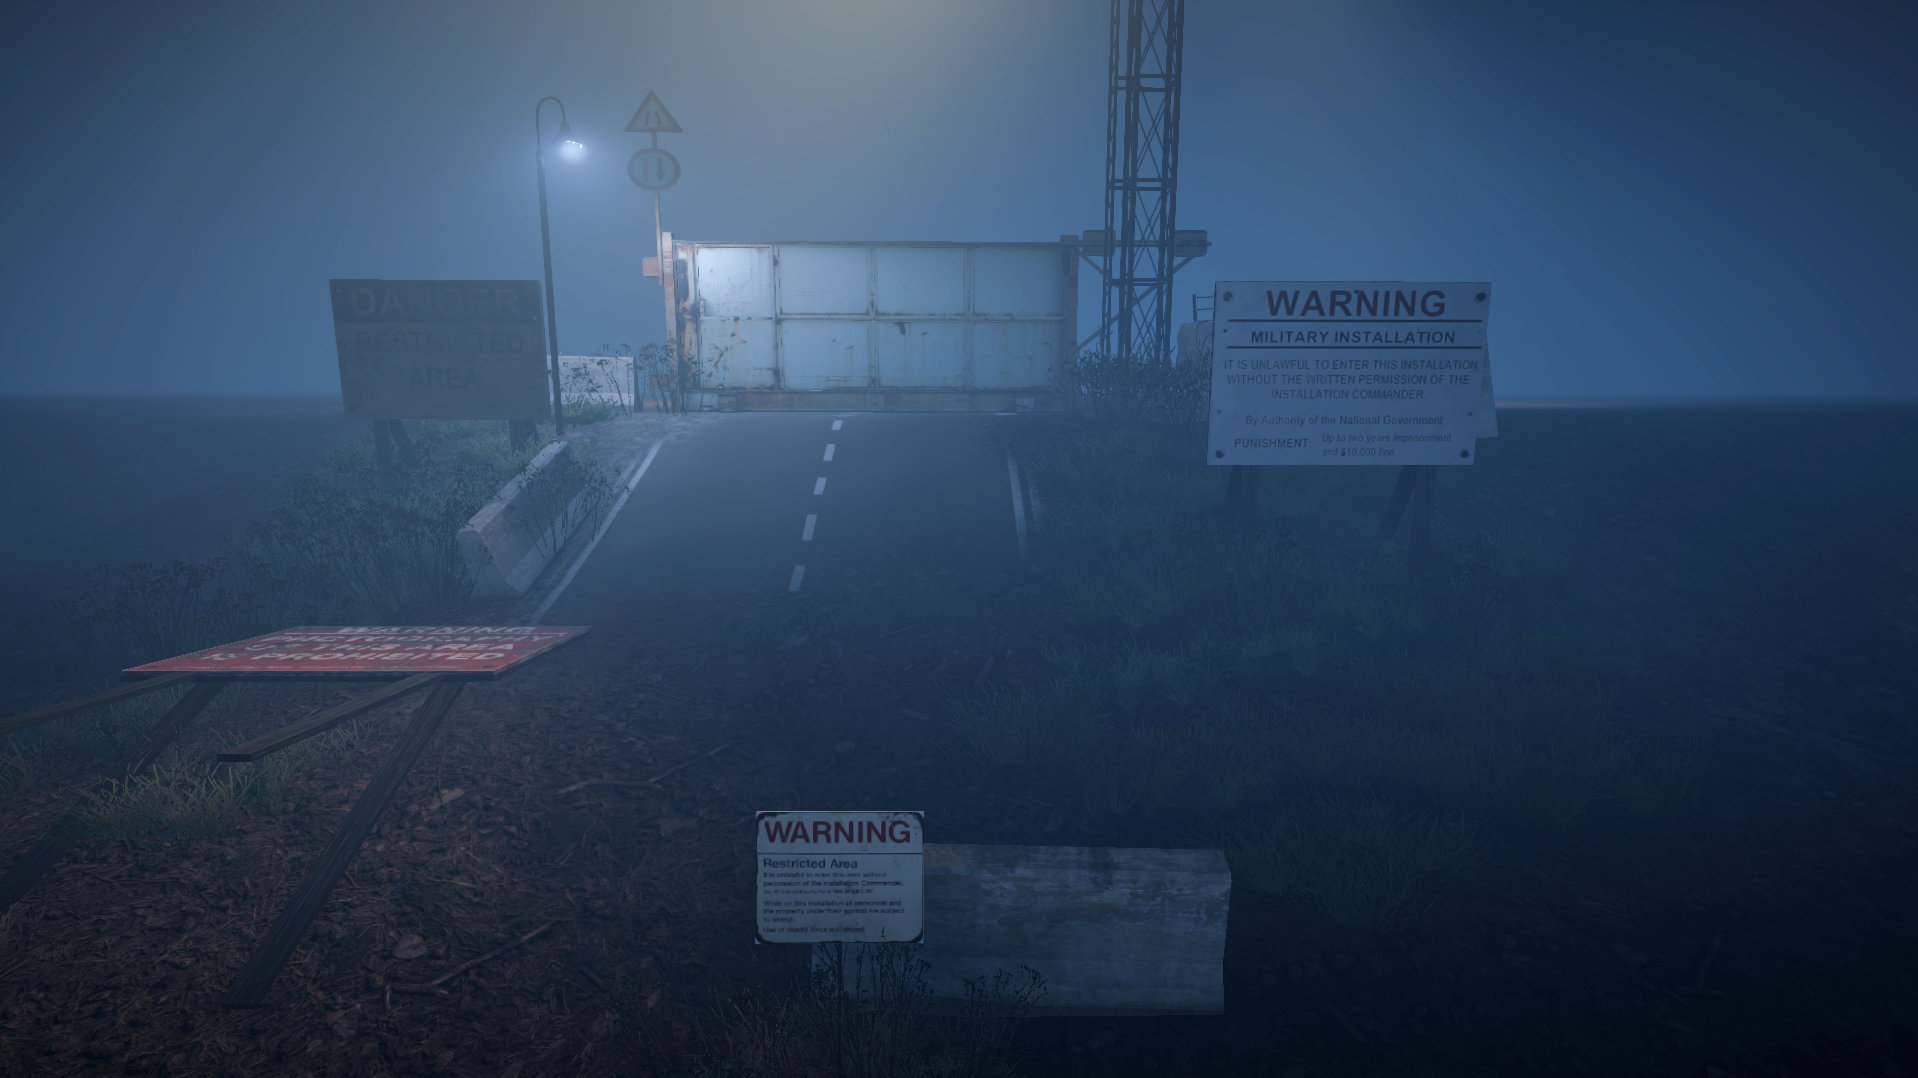
\includegraphics[width=.9\linewidth]{img/gameplay/hallo/military.png}
  \caption{Zone militaire servant de zone de transition pour le prochain chapitre}
  \label{fig:military}
\end{minipage}
\end{figure}
\end{frame}

\subsection{Chapitre 3 - Égouts}
\begin{frame}{Chapitre 3 - Égouts}
\begin{figure}
    \centering
    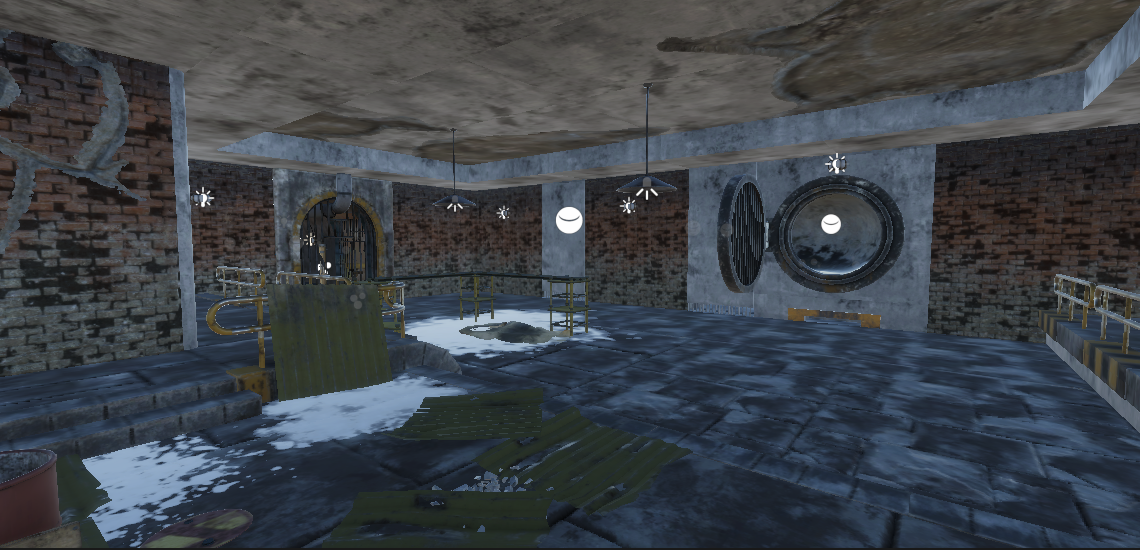
\includegraphics[width=9cm]{img/egouts/1.PNG}
    \caption{Chapitre 3: Les égouts}
    \label{fig:galaxy}
\end{figure}
\end{frame}

\begin{frame}{Chapitre 3 - Égouts - Suite}
\begin{figure}
    \centering
    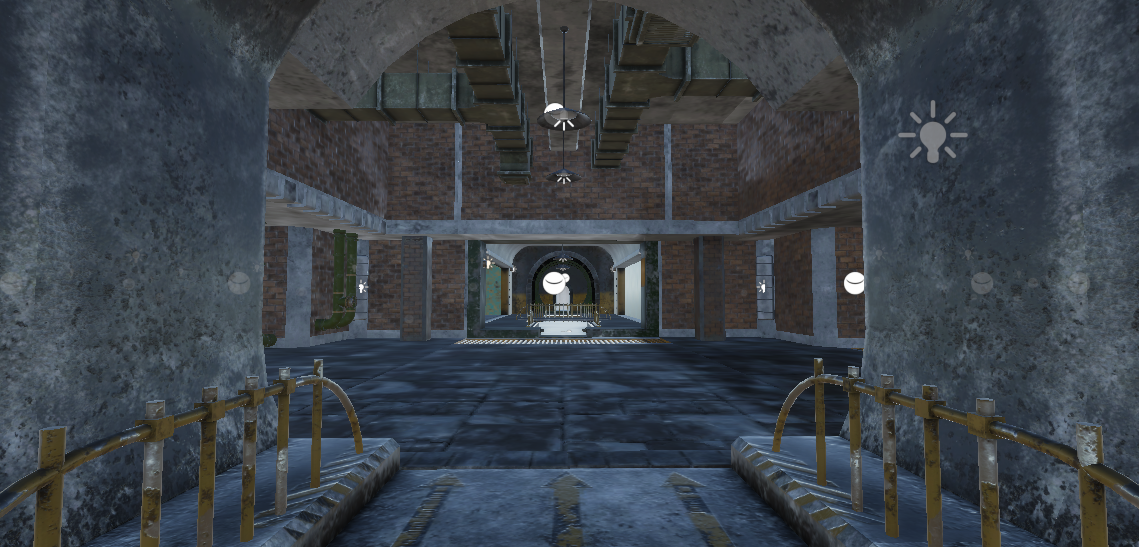
\includegraphics[width=9cm]{img/egouts/2.PNG}
    \caption{Espaces ouverts à explorer par le(s) joueur(s)}
    \label{fig:galaxy}
\end{figure}
\end{frame}

\begin{frame}{Chapitre 3 - Égouts - Suite}
\begin{figure}
    \centering
    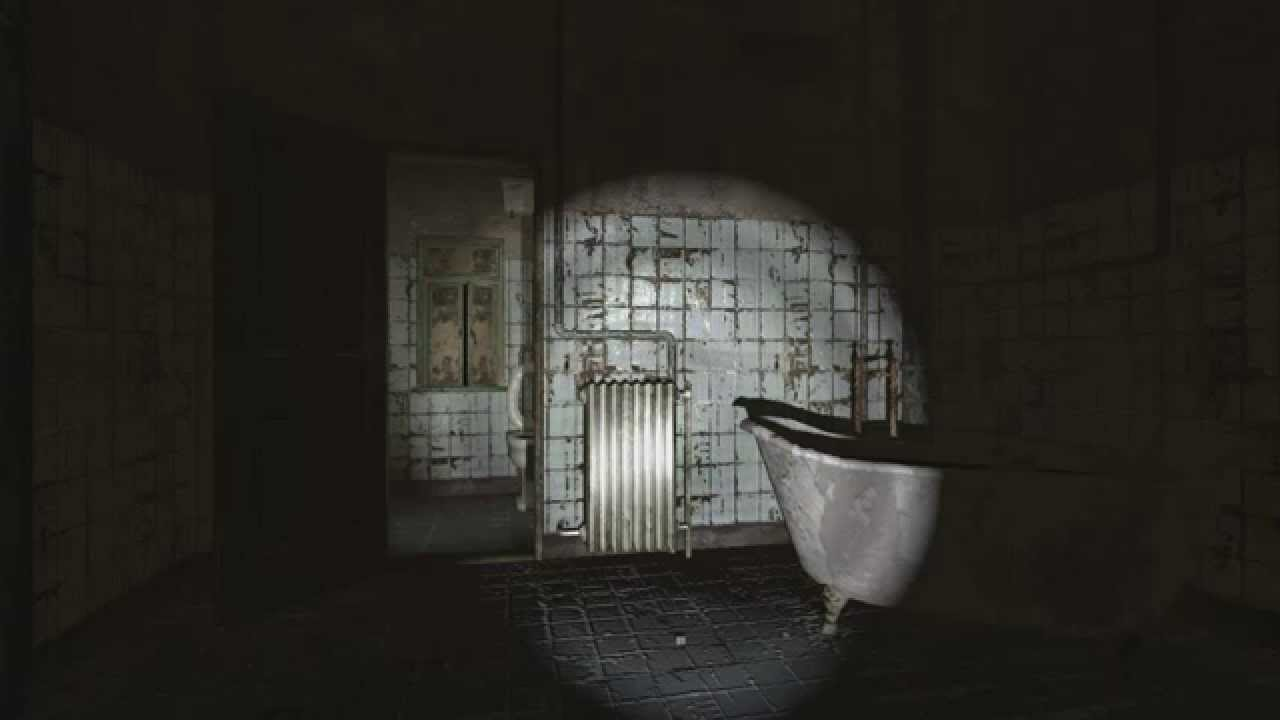
\includegraphics[width=9cm]{img/egouts/light.jpg}
    \caption{Système de lampe torche}
    \label{fig:galaxy}
\end{figure}
\end{frame}